\documentclass{article}
\usepackage{graphicx} % Required for inserting images
\usepackage[utf8]{inputenc} % Per caratteri accentati
\usepackage[T1]{fontenc}    % Per una corretta codifica dei font
\usepackage[italian]{babel} % Per sillabazione in italiano
\usepackage{float}
\usepackage{amsmath}
\usepackage{stmaryrd}
\usepackage{amsfonts}
\usepackage{mathpartir}
\usepackage{amssymb}



\title{Logica per l'informatica}
\author{}
\date{}

\begin{document}

\maketitle

\section{Formule logiche, cenni}
Alla base della logica ci sono le \textbf{proposizioni} ovvero frasi la cui validitá o meno abbia senso di essere studiata, esse nei linguaggi logico-formali (linguaggi artificiali) devono seguire una certa grammatica (\textbf{sintassi}). 
In logica formale le proposizioni vengono indicate attraverso formule logiche mentre per \textbf{enunciato} si intende una proposizione che si vuole dimostrare mediante una prova. Nonostante il termine venga usato a sproposito per \textbf{teorema}, in logica, si intende una proposizione che é stata dimostrata mediante una prova corretta: durante il processo di "prova" due sono i concetti particolarmente importanti:
\begin{itemize}
    \item \textbf{Premessa}: enunciato assunto per valido o precedentemente dimostrato
    \item \textbf{Conclusione}: enunciato che si vuole dimostrare
\end{itemize}
Il ragionamento che sta alla base della logica é il \textbf{ragionamento ipotetico} che si basa sul partire da certe ipotesi sulle quali si costruisce poi il ragionamento. Alla fine peró nonstate il ragionamento sia giusto la validitá reale di esso rimane rilegata alla veritá o meno delle premesse.


\section{Sintassi della logica di prim'ordine}
\begin{itemize}
    \item \textbf{$\perp$} (bttom): non vale
    \item \textbf{$\top$} (top): vale sempre
    \item \textbf{Predicato applicato}: può valere o non valere (es. f(n) oppure "5 é pari")
    \item \textbf{P $\land$ Q} (congiunzione): vale solo quando valgono entrambe le proposizioni
    \item \textbf{P $\lor$ Q} (disgiunzione): vale solo quando vale almeno una delle due

    \item \textbf{P $\Rightarrow$ Q} (implicazione): vale se la seconda vale sotto l'ipotesi della prima
    \item \textbf{P $\Leftrightarrow$ Q} (coimplicazione): vale se valgono p => q e q=> p
    \item \textbf{$\neg$P} (negazione): vale quando P => falso
    \item \textbf{$\forall$x.P} (quantificazione universale): vale se P vale per ogni valore di x
    \item \textbf{$\exists$x.P}(quantificazione esistenziale): vale se P vale per almeno un valore di x 
\end{itemize}

La spiegazione di questa semantica è detta \textbf{spiegzione Tarskiana}, essa utilizza gli stessi simboli della meta-logica per spiegare la logica.
I simboli riportati sono detti \textbf{connettivi} perchè date due proposizioni ne permettono di creare una terza, con \textbf{arietà} si intende il numero di proposizioni che un connettivo prende in input per creare la nuova proposizione. A questo proposito c'è una nomenclatura riguardo i vari connettivi:
\begin{itemize}
    \item \textbf{Connettivi 0-ari}: $\perp$,$\top$
    \item \textbf{Connettivo unario}: $\neg$
    \item \textbf{Connettivi binari}: $\land$, $\lor$, $\Rightarrow$, $\Leftrightarrow$
    \item \textbf{Quantificatori}: $\forall$, $\exists$
\end{itemize}
Oltre alla nomenclatura c'è anche una precedenza e associatività di questi connettivi:
\begin{center}
  $\neg$ $>$ $\land$ $>$ $\lor$ $>$ $\Rightarrow$ = $\Leftrightarrow$

\end{center}

e soprattutto sono tutti \textbf{associativi a destra}.


Per esempio:

\begin{center}
\textbf{A $\land$ $\neg$B $\lor$ C $\Rightarrow$ D $\Rightarrow$ B $\lor$ C $\lor$ E }
\end{center}

diventa

\begin{center}
\textbf{((A $\land$ ($\neg$B)) $\lor$ C) $\Rightarrow$ (D $\Rightarrow$ (B $\lor$ (C $\lor$ E))) }
\end{center}


\section{Teoria assiomatica degli insiemi}
Quando si trattò di costruire la matematica da zero gli studiosi si imbatterono nel fatto che la matematica sia un mondo ipotetico e dovettero così partire da ipotesi, esse però non avevano un riscontro materiale nella realtà, per i loro ragionamenti. Sempre nel caso specifico della matematica, le ipotesi si componevano di enti basati sulla teoria degli insiemi; gli insiemi erano definiti in maniera intuitiva e questo risultò in profondi dubbi riguardo ad essa. Attualmente la questione logica della teoria degli insiemi è stata sistemata seppur non rappresenti l'unico fondamento su cui è possibile basare la matematica.

\paragraph{Teoria degli insiemi} "tutto è un insieme" questo significa che gli insiemi contengono altri insiemi.
Questa teoria è il linguaggio macchina della matematica moderna perchè implementa tutti gli enti come insiemi particolari, oltre all'efficacia nell'implementazione degli enti riesce anche ad introdurre concetti più complessi come l'infinito. Presenta però diversi svantaggi, soprattutto a livello informatico, perchè rinuncia agli aspetti computazionali degli enti: è meno efficiente nella rappresentazione dei dati oppure nell'esempio di una funzione, essa non è più un'operazione ma un insieme di numeri.

\subsection{Teoria naive} 
Definisce l'insieme come ogni collezione di oggetti che  può essere descritta in modo che sembri ragionevole, inoltre l'insieme non deve essere per forza \textbf{omogeneo} (può contenere diversi tipi di oggetti) e può contenere altri insiemi. Gli unici \textbf{predicati di base} di questa teoria sono \textbf{appartenenza} e \textbf{uguaglianza}.

In questa teoria c'è un'intuizione che può particolarmente aiutare a capirne la logica, ovvero:

\begin{center}
    "Gli insiemi sono come scatole"
\end{center}

A questo punto si chiariscono meglio due concetti principali:
\paragraph{Appartenenza} "Se apro la scatola vedo l'elemento che ci appartiene" in altre parole un elemento X di una scatola A che è elemento di una scatola B NON è un elemento di B: se apro B vedo A, non X. Per esempio Fig. \ref{esapp}

\begin{figure} [H]
    \centering
    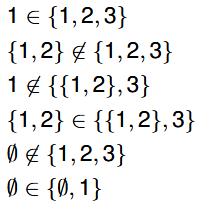
\includegraphics[width=0.25\linewidth]{es appartenenza.png}
    \caption{Esempi di appartenenza}
    \label{esapp}
\end{figure}

\paragraph{Sottinsieme} "Se aprendo le due scatole vedo gli stessi elementi" in altre parole  A è un sottoinsieme di B sse tutti gli elementi contenuti in A sono anche in B. Per esempio \ref{essott}

\begin{figure} [H]
    \centering
    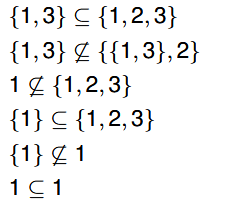
\includegraphics[width=0.25\linewidth]{es sottinsieme.png}
    \caption{Esempi di sottinsieme}
    \label{essott}
\end{figure}

Due insiemi sono uguali quando hanno gli stessi elementi, senza guardare ne l'ordine ne la ripetizione degli elementi.

\paragraph{Paradosso di Russell} sia X $=$ $\{$Y | Y $\not\in$ Y$\}$

Dunque si mostra come un elemento x $\in$ X se e solamente se x $\notin$ X, dunque si è conclusa una proposizione e il suo contrario. La matematica a questo punto si trova a dover essere basata su un'altra teoria, con l'accortezza di non utilizzare l'\textbf{assioma di comprension} peché era stato quello a generare il paradosso di Russell.

\subsection{Teorie degli insiemi assiomatica}
\begin{itemize}
    \item I connettivi primitivi (insieme, appartenenza e uguaglianza) non vengono definiti.
    \item L'esistenza di un insieme viene definita attrverso assiomi, a partire dall'esistenza di altri insiemi
    \item Di queste teorie ne esitono moltissime perché si basano su differenti assiomi
    \item Nel corso verrá seguita la teoria di \textbf{Zermelo-Fraenkel}, é la meno copntroversa e sufficiente a sviluppare la maggior parte della matematica. Inoltre non é mai stata dimostrata come inconsistente.
\end{itemize}

\subsection{Teoria Zermelo-Fraenkl}

\paragraph{Assioma di estensionalitá} Due insiemi sono uguali se e solamente se hanno gli stessi elementi.
\begin{center}
    X = Y $\Leftrightarrow$ $\forall$Z, Z $\in$ X $\Leftrightarrow$ Z $\in$ Y
\end{center}

\paragraph{Definizone di essere sottoinsieme} X é sottoinsieme di Y se Y possiede tutti gli elementi di X
\begin{center}
    X $\subseteq$ Y def. $\forall$Z, Z $\in$ X $\Rightarrow$ Z $\in$ Y
\end{center}
\textbf{N.B.} per definizione si intende un'abbreviazione di una formula lunga e complicata che abbia un significato analogo, peró mentre con un assioma restringo il campo di situazioni in cui la mia dimostrazione é vera, con la definizione non vario le casistiche ma é una mera abbreviazione.


\paragraph{Assioma di separazione} Dato un insieme posso formare dei suoi sottoinsiemi con elementi che soddisfano certe proprietà.
\begin{center}
    $\forall X,\exists Y,\forall Z(Z \in Y \Leftrightarrow Z \in X \land P(Z)$
\end{center}
Se però indico $Y= \{W \in X | P(W)\}$, allora ho una modifica dell'assioma più facile da usare:
\begin{center}
    $\forall X, \forall Z(Z\in \{W\in X|P(W)\} \Leftrightarrow Z \in X \land P(Z))$
\end{center}

Anche in questo caso si può simulare il \textbf{Paradosso di Russell} ($X=\{Y\in U | Y\notin Y\}$) ma in questo caso quello che era l'insieme U (collezione di insiemi) non è un insieme ma una \textbf{classe}.


\paragraph{Assioma dell'insieme vuoto}
\begin{center}
    $\exists X,\forall Z, Z \notin X$
\end{center}

Se dunque $X=\emptyset$ allora $\forall Z, Z \notin X$

A questo punto si può introdurre anche una \textbf{Definizione di insieme vuoto} perchè partendo dall'assioma di un qualsiasi insieme allora l'insieme vuoto può sempre essere definito come sottoinsieme di esso:
\begin{center}
    $\emptyset = \{X \in Y |false\}$
\end{center}
infatti, dall'assioma di separazione 
\begin{center}
    $Z \in \{X\in Y|false\} \Leftrightarrow Z\in Y \land false \Rightarrow false$ da cui $Z \notin \emptyset$
\end{center}

\paragraph{Definizione di intersezione}
\begin{itemize}
    \item \textbf{Binaria} $A\bigcap B = \{ X\in A |X\in B\}$
    dunque posso dire che $X\in A\bigcap B \Leftrightarrow X\in A \land X\in B$
    \item \textbf{N-aria} $A_1\bigcap...\bigcap A_n = (...((A_1\bigcap A_2)\bigcap A_3)...\bigcap A_n)$
\end{itemize}
Tuttavia l'assioma per l'intersezione n-aria \textit{NON} permette di avere $n=\infty$.
Esiste anche peró un modo piú compatto utilizzando un insieme che contiene gli insiemi che si voglio intersecare:

\begin{center}
    $F$=insieme di insiemi
    
    $\bigcap F$= insieme delle intersezioni

    $\bigcap F = \emptyset$ se $F=\emptyset$  (scelta non usuale perché $\emptyset$ nopn é l'elemento neutro di questa operazione.

    $\bigcap F= \{X\in A | \forall Y, (Y\in F \Rightarrow X\in Y0\}$ con $A\in F$
\end{center}
Fig.\ref{intersezione}

\paragraph{Assiome dell'unione} 
\begin{center}
    $F$ = insieme degli insiemi che si vuole unire


    $\bigcup F= \forall F,\exists X, \forall Z,(Z\in X \Leftrightarrow Z\in A \land Z\in B)$ in questo caso $X=\bigcup F$.

\end{center}

\textbf{Teorema dell'unione binaria}: 
\begin{center}
    $\forall A, \forall B, \exists X, \forall Z,(Z\in X \Leftrightarrow Z\in A \lor Z\in B)$
\end{center}
Quindi se $A\bigcup B$ allora $\forall A, \forall B, \forall Z, (Z\in A\bigcup B \Leftrightarrow Z\in A \lor Z\in B)$

\paragraph{Asioma del singoletto} Per singoletto si intende un insieme di un solo elemento.
\begin{center}
    $\forall X,\exists Y,\forall Z(Z \in Y \Leftrightarrow Z = X)$
\end{center}


Questo assioma permette di avere un'infinitá di insiemi, infatti: 
$\emptyset \not = \{\emptyset\} \not = \{\{\emptyset\}\} ...$ e cosí avanti con sempre piú singoletti.

$\{\{\emptyset\}\} \bigcup \{\emptyset\} = \{\{\emptyset\}, \emptyset\}$ e cosí avanti si possono ottenere \textbf{infiniti insiemi finiti}.

\textbf{Notazione}: con $\{A_1 ... A_n\}$ si indica l'insieme $\{A\} \bigcup ...\bigcup \{A_n\}$


\paragraph{Costruzione dei numeri naturali} Per ogni meta-numero naturale n definisco un insieme $\llbracket n \rrbracket$:


\begin{center}
    $\llbracket n \rrbracket = \emptyset$

    $\llbracket n +1\rrbracket = \llbracket n \rrbracket \bigcup \{\llbracket n \rrbracket\}$
\end{center}

Da questa definzione di puó fare l seguente osservazione: $n =  \{0,...,n-1\}$, ne segue che: 


\begin{center}
$n\leq m \Leftrightarrow n\in m$

$MAX(n,m) = n \bigcup m$

$MIN(n,m) = n\bigcap m$
\end{center}


Ma questa definizione é corretta? Bisogna vedere quali proprietá dei numeri si vogliono preservare, in questo caso si vuole mantenere la differenza tra tutti i numeri.


\begin{figure}[H]
    \centering
    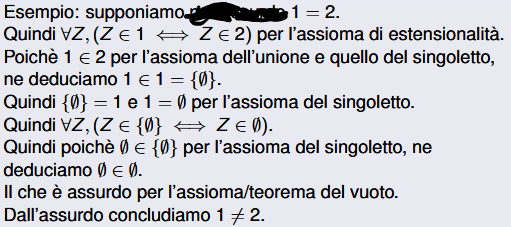
\includegraphics[width=0.75\linewidth]{Numeri diversi.png}
    \caption{Dimostrazione che ogni numero é diverso da un altro (a coppie)}
    \label{numeri diversi}
\end{figure}



\paragraph{Assioma di infinito (contiene almeno tutti i naturali)}
\begin{center}
    $\exists Y,(\emptyset\in Y \land \forall N(N\in Y \Rightarrow N \bigcup \{N\}\in Y))$
\end{center}

\paragraph{Assioma dell'insieme potenza} Afferma che esiste l'insieme dei sottoinsiemi di un dato insieme

\begin{center}
$\forall X,\exists Y,\forall Z(Z\in Y \Leftrightarrow Z\subseteq X)$
\end{center}

$Y$ lo posso scrivere come $Z^X$ o $P(X)$ ed é l'insieme potenza o insieme delle parti: 

$2^{\{1,2\}} = \{\emptyset, \{1\}, \{2\}, \{1,2\}\} = 4$

\paragraph{Assioma di regolaritá o fonazione}
\begin{center}
    $\forall X\not= \emptyset$ ha un elemento dal quale é \textbf{disgiunto}.
\end{center}
Come conseguenza nessun insieme contiene ricorsivamente sé stesso dunque ha senso misurare e confrontare la cardinalitádelgi insiemi.

\paragraph{Assioma di rimpiazzamento} L'immagine di un insieme rispetto ad una formula che descrive una funzione é ancora un \textbf{insieme}.

\section{Dimostrazioni}
Sono regolate da un linguaggio artificiale, quelle informali saranno delle approssimazioni meno verbose di quelle informali e soprattutto ogni dimostrazione é finita. La finalità di una dimostrazione è quella di trasferire ad un'altra persona un'intuizione personale: Per studiare la logica si faranno dimostrazioni che nella metalogica sono considerate informali.

\subsection{Per ogni ($\forall$)}
\paragraph{Introduzione} si va a lavorare sulla conlusione: prendo un X qualsiasi, che peró non varia durante la dimostrazione, e ne dimostro la prprietá P(X). Cosí facendo per in qualsiasi caso specifico di X so che P(X) varrá. In lean si implementa con [assume x : set...].
\paragraph{Eliminazione} si lavora su quello che si sa: si sceglie un particolare X dato che P(X) vale $\forall$ X. In lean si implementa con: [by "nome ipotesi" we proved "conclusione" as "nome nuovo risultato intermedio"]

\subsection{Implicazione ($\Rightarrow$)}
\paragraph{Introduzione} assumo che P valga e passo a dimostrare Q. In lean [suppose P as H], con H ipotesi.
\paragraph{Eliminazione} sapendo che P $\Rightarrow$ Q allora so che in qualsisi momento della dimostrazione in cui dimostro che valga P posso concludere che anche Q valga. In lean [by "nome ipotesi PQ", "nome ipotesi P" we proved "Q"]
\paragraph{Eliminazione, variante} Chiamando H un risultato intrmedio di P $\Rightarrow$ Q per dimostrare Q basta torare a dimostrare P. In lean [by H it suffices to prove P]
\subsection{Coimplica ($\Leftrightarrow$)} 

\paragraph{Introduzione} per dimostrare che P $\Leftrightarrow$ Q, devo dimostrare sia P $\Rightarrow$ Q che Q $\Rightarrow$ P. In lean [we split the proof]
\paragraph{Eliminazione} sapendo che P $\Leftrightarrow$ Q allora possiamo usar che P $\Rightarrow$ Q e Q $\Rightarrow$ P.



\textbf{Convenzione} (non in lean):  quando in un enunciato compaiono delle variabili non dichiarate da $\forall$ si considerano comunque introdotte da $\forall$.

\subsection{Esplicitazione della conclusione} (metodico, non logico) Letteralmente "dobbiamo dimostrare P" perché conviene esplicitare cosa si sta/resta da dimostrare. 
In lean [we need to prove P]

\subsection{Ovvio} Qundo il lettore è in grado di ricostruire la dimostrazione per conto suo, per esempio combinando le ipotesi. (molto arbitrario)
In lean: [done].

\subsection{Abbreviazioni} 
\paragraph{Da $H_1$, ..., $H_n$} quando si dimostra una certa proprietá P(H) con tutti gli elementi H. In lean [by $H_1$, ..., $H_n$ we proved P as H].

\subsection{Quindi} Insieme ad altri sinonimi sono il modo per fare riferimento all'ultima ipotesi o risultato intermedio.
\subsection{Espansione di definizione} Usato per espandere la definizione P in modo da arrivare a Q. In lean [P that is equivalent to Q].

\subsection{Assurdo ($\perp$)}
\paragraph{Introduzione} non esiste
\paragraph{Eliminazione} ci si concentra su casi impossibili per cui si può concludere qualsiasi cosa, infatti a livello pratico arrivando ad un $\perp$ si può dimostrare qualsiasi proposizione, Fig(\ref{dimass}). In Lean [by "nome" done].

\subsection{Negazione ($\neg$)} $\neg P$ è un'abbreviazione di $P\Rightarrow \perp$ quindi si svolge come caso particolare dell'implicazione; a livello pratico per dimostrare $\perp P$ si assuma $P$ e si dimostra un \textbf{assuro}, importante è ricordare che \textbf{non è una dimostrazione per assurdo}. 

\subsection{Congiunzione ($\land$)}
\paragraph{Introduzione} per dimostrare $P \land Q$ si dimostra prima P poi Q.
\paragraph{Eliminazione} si possono usare P e Q come ipotesi (Fig. \ref{cong1})

\subsection{Disgiunzione ($\lor$)}
\paragraph{Introduzione} per dimostrare $P\lor Q$ si sceglie di dimostrare una delle due proposizione. (Fig.\ref{disint})
\paragraph{Eliminazione} partendo da $P\lor Q$ si dimotra per casi: una volta assumendo che solo P valga e l'altra assumendo che solo Q valga

\subsection{Risultati intermedi} nel mezza di una dimostrazione si puó introdurre un risultato intermedio che serve per lo svolgimento della dimostarzione. (Fig. \ref{risint})

\subsection{Esiste ($\exists$)}
\paragraph{Introduzione}: per dimostare che $\exists X, P(X)$ si sceglie un certo insieme $E$ e si dimostra $P(E)$; essendo dunque $E$ un insieme qualunque bisogna prestare attenzione a sceglierlo in maniera corretta per il fine della dimostarzione. (Fig. \ref{esiste})
\paragraph{Eliminazione} sapendo che $\exists X,P(X)$ si introduce unípotesi che peró non deve essere giá stata utilizzata. (Fig. \ref{esiste})


\section{Esempi di dimostrazioni}
\begin{figure} [h!]
    \centering
    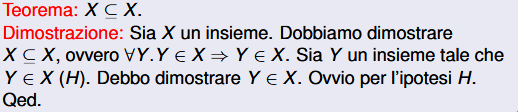
\includegraphics[width=0.8\linewidth]{Riflessivita di c.png}
    \caption{Dimostrazione riflessivitá $\in$}
    \label{rifc}
\end{figure}

\begin{figure}[h!]
    \centering
    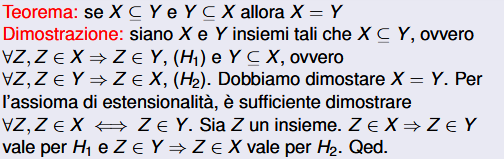
\includegraphics[width=0.8\linewidth]{Anti simm di c.png}
    \caption{Dimostrazione anti-simetria di $\in$}
    \label{antisimc}
\end{figure}

\begin{figure}[H]
    \centering
    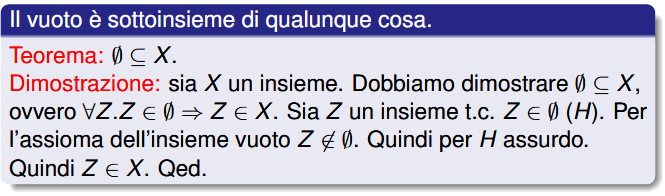
\includegraphics[width=1\linewidth]{Dimconass.png}
    \caption{Dimostrazione $\emptyset$ è sottoinsieme si qualsiasi insieme}
    \label{dimass}
\end{figure}

\begin{figure}[H]
    \centering
    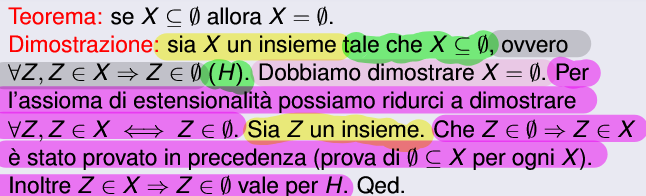
\includegraphics[width=0.85\linewidth]{Unico sottoinsieme del vuoto e il vuoto.png}
    \caption{L'unico sottoinsieme dell'insieme vuoto é il vuoto stesso}
    \label{vuoto}
\end{figure}


\begin{figure} [H]
    \centering
    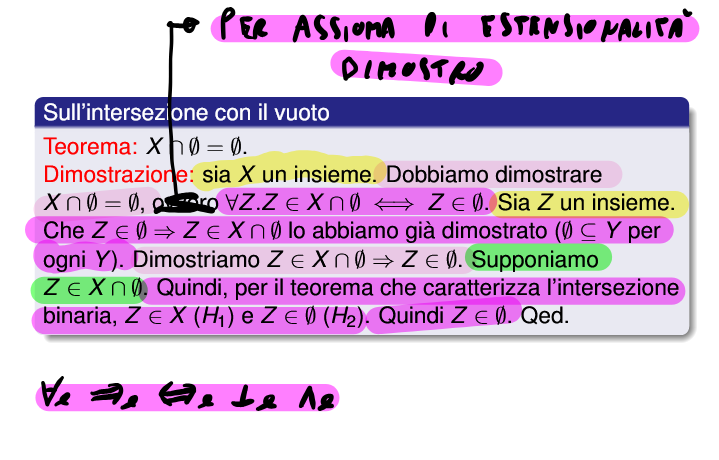
\includegraphics[width=0.75\linewidth]{Cong 1.png}
    \caption{Esempio di eleiminazione della congiunzione}
    \label{cong1}
\end{figure}

\begin{figure} [H]
    \centering
    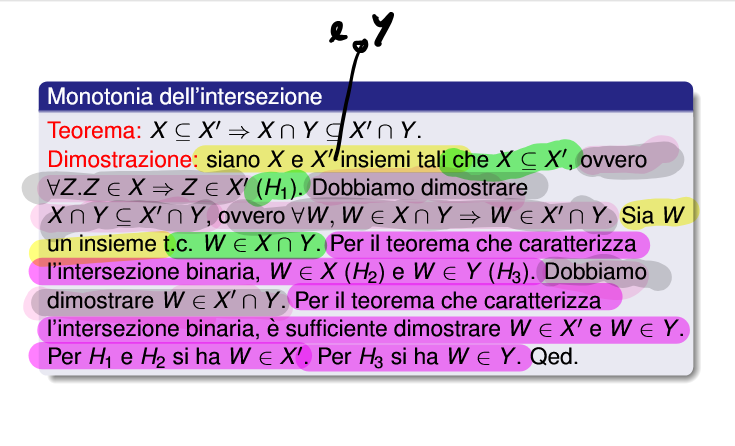
\includegraphics[width=0.75\linewidth]{mon int.png}
    \caption{}
    \label{intersezione}
\end{figure}

\begin{figure} [H]
    \centering
    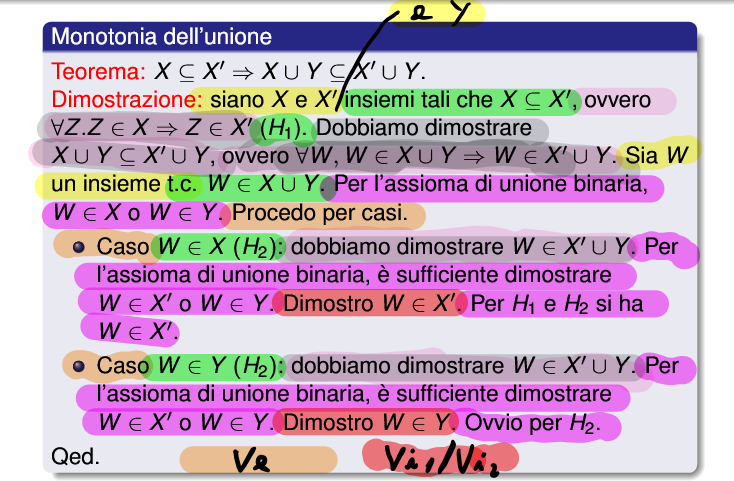
\includegraphics[width=0.75\linewidth]{disint.png}
    \caption{Esempio di introduzione della disgiunzione}
    \label{disint}
\end{figure}

\begin{figure} [H]
    \centering
    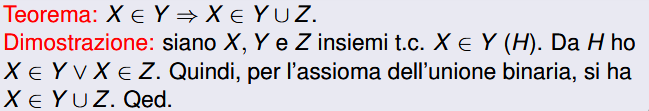
\includegraphics[width=0.75\linewidth]{Ris int.png}
    \caption{Esempio dell'utilitá di utilizzare risultati intermedi}
    \label{risint}
\end{figure}


\begin{figure} [H]
    \centering
    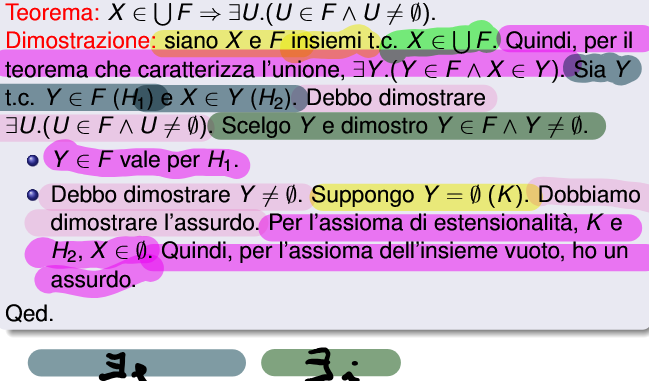
\includegraphics[width=0.75\linewidth]{esies.png}
    \caption{Esempio di introduzione e eliminazione dell'esistenza}
    \label{esiste}
\end{figure}


\section{Logica}
Si pongono le basi della matematica sulla teoria degli insiemi

\paragraph{Coppie ordinate} Formate da due componenti in cui l'ordine degli elementi é importante (n.b. non é l'insieme dei suoi elementi).

\begin{center}
    $X,Y$ sono una \textbf{coppia ordinata} $[(X,Y)]$ é l'insieme $\{X,\{X,Y\}\}$

    $\langle X,Y\rangle$ = $\langle X^{'},Y^{'}\rangle \Leftrightarrow  X = X^{'}$  $Y = Y^{'}$

    Corollario:  $\langle X,Y\rangle \not= \langle X^{'},Y^{'}\rangle$ $\Leftrightarrow$  $X\not= Y$
\end{center}


\paragraph{Prodotto caretesiano [$A\times B$]}
\begin{center}
    $\forall A,\forall B, \exists X,\forall Z(Z\in C \Leftrightarrow\exists a,\exists b,( a\in A \land b\in B \land Z =\langle a,b\rangle))$
\end{center}

\paragraph{Definizione di relazione} Un qualunque insieme sottoinsieme di $A\times B$:
\begin{center}
    Sia \textit{R} una relazione $a$\textit{R}$b \Leftrightarrow\langle a,b\rangle \in $ \textbf{R}
\end{center}

\begin{figure}[H]
    \centering
    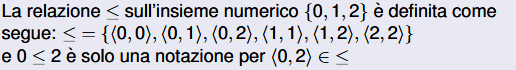
\includegraphics[width=0.75\linewidth]{Esrelazione.png}
    \caption{Esempio dell'applicazione della definizione di relazione}
    \label{reled}
\end{figure}

\textbf{Teorema delle relazioni da/verso insiemi vuoti}:

Se \textit{R}$\subseteq A\times \emptyset$ oppure $ \textit{R}\subseteq\emptyset\times A  \Rightarrow \textit{R} = \emptyset$.

\paragraph{Definizione di funzione} Detti A \textbf{dominio} e B \textbf{codominio} la funzione é una qualsiasi relazione $f\subseteq A\times B |\forall x(x\in A \Rightarrow\exists!Y, xfy)$

\textbf{Notazione}: $y = f(x) \rightarrow \langle x,y\rangle\in f$

\textbf{Teorema dell'esistenza dello spazio di funzione come insieme}

$\forall A,\forall B,\exists c, \forall f(f\in c\Leftrightarrow f$ é funzione di dominio $A$ e codominio $B)$

$C = B^A$ é lo spazio della funzione da A a B.

\begin{figure}[H]
    \centering
    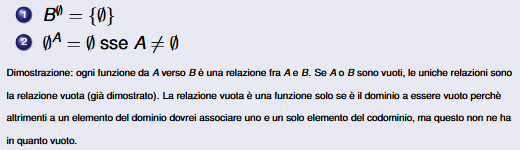
\includegraphics[width=0.95\linewidth]{Dimfunznull.png}
    \caption{Funzioni da/verso insiemi vuoti}
    \label{sunzinsnull}
\end{figure}

\paragraph{Quantificazione limitata}
Ovvero delle abbreviazioni nella notazione
\begin{enumerate}
    \item $\forall x \in A, P(X)$ indica $\forall x(x \in A \Rightarrow P(X))$
    \item $\exists x \in A, P(X)$ indica $\exists x(x \in A \land P(X))$
    \item $\forall x, y \in A, P(x,x)$ indica $\forall x \in A, \forall y\in A, P(x,y) $
    \item $\exists x,y \in A, P(x,y)$ indica $\exists x \in A, \exists y\in A, P(x,y) $
\end{enumerate}

\paragraph{Proprietá delle relazioni}
\begin{enumerate}
    \item \textbf{Riflessivitá}: se $\forall x\in A, x\textit{R}x$
    \item \textbf{Simmetria}: se $\forall x,y\in A,(x\textit{R}y \Rightarrow y\textit{R}x)$
    \item \textbf{Transitivitá}: se $\forall x,y,z\in A, (x\textit{R}y \land y\textit{R}z \Rightarrow x\textit{R}z)$
\end{enumerate}

\paragraph{Relazione di ordinamento stretto}
$\textit{R} \subseteq A\times A$ é un relazione di ordinamento stretto se e solamente se é sia \textbf{transitiva} che \textbf{riflessiva}.

\paragraph{Relazione di ordinamento (lasca)}
$\textit{R} \subseteq A\times A$ é un relazione di ordinamento (lasca) se e solamente se é \textbf{transitiva}, \textbf{riflessiva} e \textbf{antisimmetrica}.
Una relazione é \textbf{antisimmetrica} $\Leftrightarrow \forall x,y\in A, (x\textit{R}y \land y\textit{R}x \Rightarrow x=y)$

\paragraph{Relazione di equivalenza ($\equiv$)}
Una relazione é di equivalenza se e solamente se é sia \textbf{riflessiva} che \textbf{simmetrica} e \textbf{transitiva}. Intuitivamente é prendere un insieme e mettere in relazione tra di loro tutti gli elementi che hanno una certa caratteristica volutamente scartandone altre (Fig.\ref{esclaequi}).

\paragraph{Classi di equivalenza}
Sia $\equiv \subseteq A\times A$ una relazione di quivalenza su A, la \textbf{classe di equivalenza} di $x\in A$ rispetto a $\equiv$ é:
\begin{center}
    $[x]_\equiv = \{y \in A | y \equiv x\}$
\end{center}

\textbf{Teorema}: sia $\equiv\subseteq A\times A, \forall x,y \in A$ si possono verificare due situazioni: o le due classi si equivalenza sono uguali($[x]_\equiv = [y]_\equiv\Rightarrow x\equiv y$) oppure sono due insiemi disgiunti $([x]_\equiv \not= [y]_\equiv \Rightarrow x\not\equiv y$) (Fig.\ref{dimclaequiv}).

\begin{figure} [H]
    \centering
    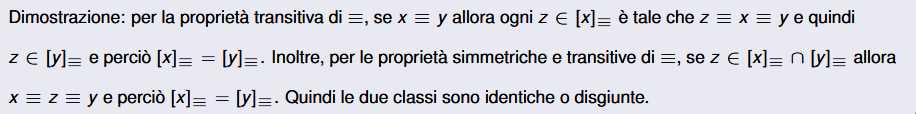
\includegraphics[width=1.15\linewidth]{Dimclassequiv.png}
    \caption{Dimostrazione del teorema delle classi di equivalenza}
    \label{dimclaequiv}
\end{figure}

\begin{figure}[H]
    \centering
    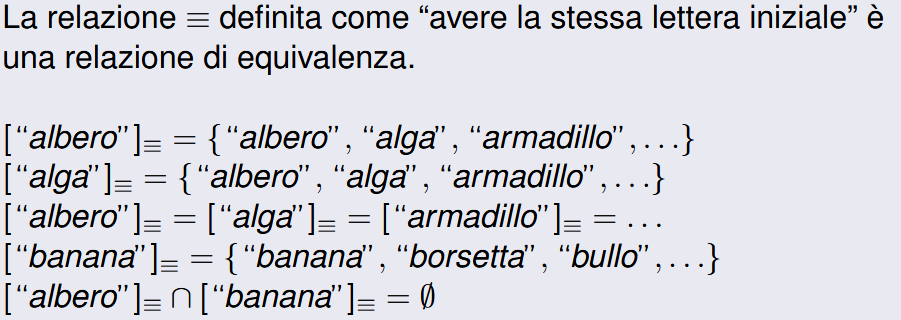
\includegraphics[width=0.75\linewidth]{esclaequiv.png}
    \caption{Esempio di classi di equivalenza}
    \label{esclaequi}
\end{figure}

\paragraph{Insieme quoziente}
É l'isieme di tutte le classi equivalenti rispetto ad un certo $x$, ovvero delle classi equivalenti di ogni possibile $x$.

Sia $\equiv \subseteq A\times A$ allora $A_{\textbackslash\equiv} = \{[x]_\equiv|x\in A\}$ essendo peró un insieme di insiemi sará dunque una classe.



\paragraph{Costruzione dell'insieme dei numeri interi ($\mathbb{Z}$)}
Questa costruzione é necessaria per rendere la sottrazione tra naturali sempre possibile qualsiasi sia la coppia di nuemri. Introduco dunque un insieme $Z = \mathbb{N}\times\mathbb{N}$, sapendo giá come funziona la matematica so che la sottrazione tra le seguenti coppie $\langle 2,4\rangle \in Z = 2-4$ e $\langle 3,5 \rangle \in Z = 3-5$ é uguale quindi per renderlo formale prima vanno rese equivalenti e poi vanno quozientate per renderle uguali. Per fare ció tango in considerazione che $2 -4 \equiv 3 - 5 \not\in \mathbb{N}$ ma $2 + 5 \equiv 3+4 \in \mathbb{N}$ quindi definico $\equiv\subseteq Z\times Z : \langle u_1, l_1 \rangle \equiv \langle u_2, l_2\rangle \stackrel{\mathrm{def}}{=} u_1 + l_2= u_2 l_1$. Arrivato dunque alla relazione di equivalenza la quozione e definisco i numeri interi come $\mathbb{Z} \stackrel{\mathrm{def}}{=} Z_{\textbackslash \equiv}$, quindi per come é stato definito $\mathbb{N} \not\subseteq\mathbb{Z}$.


\paragraph{Nozione di infinito}
Per comprendere meglio la nozione di infinito é opportuno introdurre prima le \textbf{proprietá delle funzioni} ($f: B^A$):
\begin{itemize}
    \item \textbf{Iniettivitá}: $\forall a,b\in A, \Rightarrow f(a) = f(b) \Rightarrow a = b$
    \item \textbf{Suriettivitá}: $\forall y\in B, \exists x\in A | f(x) = y$
    \item \textbf{Biettivitá}: quando una funzione é iniettiva e suriettiva.
\end{itemize}
Giá queste proprietá possono dire molto sulla "grandezza" dei due insiemi: se una funzione é iniettiva allora $B \geq A$, se invece una funazione é suriettiva allora $A \geq B$; infine se una funzione é biettiva allora $A=B$.

\paragraph{A e B hanno la stessa cardinalitá}  $\stackrel{\mathrm{def}}{=} \exists Biezione (A,B)$, questa definizione ha una conseguenza importante: volendo introdurre una relazione di equivalenza tra due insiemi bisogna introdurre una classe che li contenga.

Sia $U$ la classe degli insiemi, un numero cardinale é un elemento di $U_{\textbackslash\equiv}$ dove per $\equiv$ si intende avere la stessa cardinalitá.

\paragraph{Questioni insiemistiche importanti}

Dunque si puó affermare che $\mathbb{N}\equiv \mathbb{Z}?$
Per farlo devo costruire una funzione biettiva tale che $f:\mathbb{N} \rightarrow \mathbb{Z} $

$f(x)$
$\begin{cases}
    -\frac{n}{2} & \text{se n pari}\\
    \frac{n+1}{2}& \text{se n dispari}
\end{cases}$

Avendo cosí costruito la fuinzione con le caratteristiche sopra descritte posso affermare che $\mathbb{N}\equiv \mathbb{Z}$


Posso fare lo stesso per $\mathbb{N}\equiv \mathbb{Q}?$. (Fig\ref{Qdim})

\begin{figure}[H]
    \centering
    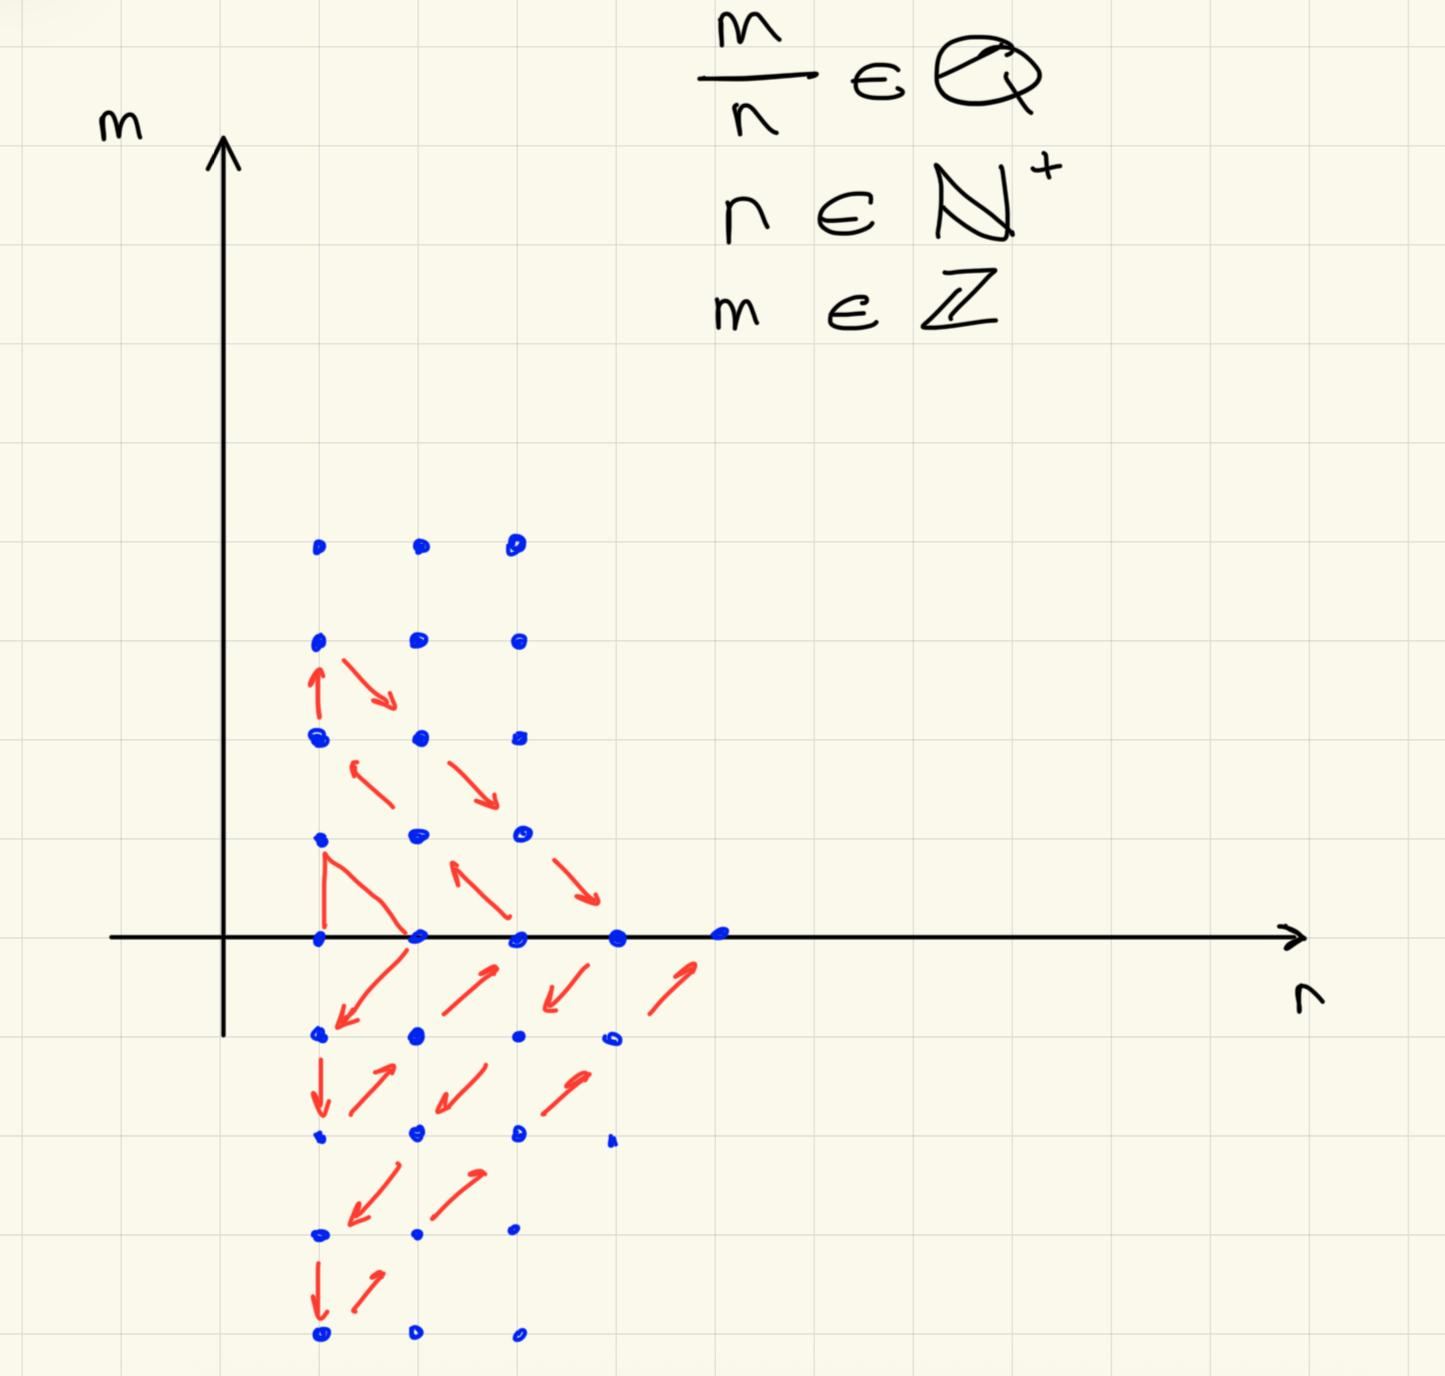
\includegraphics[width=0.65\linewidth]{dimQ.jpg}
    \caption{Dimostrazione dell'enumerabilitá di Q}
    \label{Qdim}
\end{figure}


E invece per $\mathbb{N}\equiv \mathbb{R}?$

Grazie a \textbf{Cantor} é stato dimostrato che $\mathbb{N}\not\equiv \mathbb{R}$, per semplicitá mi limito a dimostarre che $\mathbb{N}\not\equiv [0,1]\subseteq\mathbb{Z}$ partendo peró da $\mathbb{N}\equiv [0,1] \Rightarrow \exists f\in [0,1]$ e dimostro un assurdo:

$m\in [0,1] = 0.d_0 d_1d_2...$ con $d_i\in\{0,1,2,3...,9\}$

$\begin{aligned}
f(0) &= d_0^0 \cdot d_1^0 \cdot d_2^0 \cdot d_3^0 \cdot d_4^0 \\
f(1) &= d_0^1 \cdot d_1^1 \cdot d_2^1 \cdot d_3^1 \cdot d_4^1 \\
f(2) &= d_0^2 \cdot d_1^2 \cdot d_2^2 \cdot d_3^2 \cdot d_4^2 \\
f(3) &= d_0^3 \cdot d_1^3 \cdot d_2^3 \cdot d_3^3 \cdot d_4^3 \\
f(4) &= d_0^4 \cdot d_1^4 \cdot d_2^4 \cdot d_3^4 \cdot d_4^4 \\
f(5) &= d_0^5 \cdot d_1^5 \cdot d_2^5 \cdot d_3^5 \cdot d_4^5
\end{aligned}$



A questo punto creo il mio numero $r = \bar{d_0^0} \bar{d_1^1}\bar{d_2^2}...$ con $\bar{d_i^i \not\in \{9,d_i^i\}}$ in modo tale da essere sempre diverso da ogni possibile $f(x)$. Quindi si é giunti ad un assurdo.


\paragraph{Cardinalità di un insieme (|A|)} E' una funzione che restituisce il \textbf{numero cardinale} $[A]_{\backslash\equiv}$

\paragraph{Definizione di insieme finito} Un insieme si dice finito $\Leftrightarrow$ non è un insieme infinito.

\paragraph{Albergo Hilbert} Immagina un albergo di infinite stanza che però possono solo ospitare un ospite, se arriva un nuovo cliente lo si può mettere in una stanza. Se invece l'albergo fosse finito e già tutto occupato non si potrebbe aggiungere nessun cliente.

\paragraph{Insieme infinito} E' un insieme che è in bisezione con un suo sottoinsieme proprio ($B\subsetneq A \land |B|=|A|$)

\paragraph{$\leq$ sui numeri cardinali} Dati $x,y$ numeri cardinali tali che $|A| = x, |B| = y$ se c'è un'iniezione fra A e B allora $A\leq B$

\paragraph{$<$ sui nuomeri cardinali} Se $X \leq Y \land X \not= Y$


\paragraph{Enunciato del teorema di Cantor} Sia $T$ non vuoto, allora $|T| < |2^T|$ (insieme delle parti)

\paragraph{Corollario del teorema di Cantor} $\forall T $ tale che $ |T|>2$ allora $|T| <|T^T|$

\paragraph{Big problem} In informatica però non si può rappresentare l'infinito e tutte le funzioni che lo implicano (in realtà nemmeno tutte le funzioni possibili), per cui verranno adottate 2 soluzioni:
\begin{enumerate}
    \item Evitano insiemi generici e funzioni matematiche andando a lavorare su dati finiti
    \item Uso di linguaggi artificiali per evitare paradossi logici.
\end{enumerate}



\section{Deduzione naturale}
Studia gli \textbf{alberi di deduzione naturale} attraverso la \textbf{logica proposizionale}, cioè una logica che è più ristretta rispetto a quella già vista ma è molto utile in informatica perchè studia "Tutto ciò che può essere scritto come proposizione"

\begin{figure}[H]
    \centering
    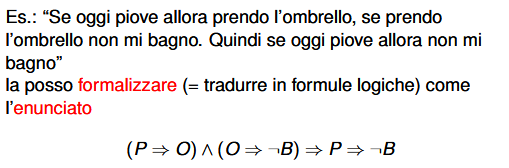
\includegraphics[width=0.75\linewidth]{eslogprep.png}
    \caption{Esempio di formalismo della logica proposizionale}
    \label{loprop}
\end{figure}

\paragraph{Sintassi}
\begin{itemize}
    \item \textbf{$\perp$} (bttom): non vale
    \item \textbf{$\top$} (top): vale sempre
    \item \textbf{P $\land$ Q} (congiunzione): vale solo quando valgono entrambe le proposizioni
    \item \textbf{P $\lor$ Q} (disgiunzione): vale solo quando vale almeno una delle due

    \item \textbf{P $\Rightarrow$ Q} (implicazione): vale se la seconda vale sotto l'ipotesi della prima
    \item \textbf{$\neg$P} (negazione): vale quando P => falso
    \item \textbf{$A,B...$}: variabili proposizionali che possono valere o meno
\end{itemize}

Inoltre si definisce $F$ un formula quando la si vuole dimostrare (ovvero é la conclusione) e $\Gamma$ un insieme di formule di partenza (ovvero le ipotesi); se $\Gamma\vdash F$ (gamma deriva F) se ho un \textbf{albero di deduzione naturale}.

\begin{figure}[H]
    \centering
    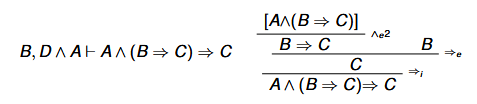
\includegraphics[width=0.95\linewidth]{esalbero.png}
    \caption{Esempio di albero di deduzione natuale}
    \label{esalbe}
\end{figure}

\paragraph{Quali sono i requisiti per essere un albero?}
\begin{itemize}
    \item I nodi devono essere formule
    \item Le foglie sono formule scaricate/cencellate (\textbf{ipotesi locali})e sono scritte tra [] oppure sono formule non scaricate ovvero \textbf{ipotesi globali}
    \item La radice è \textbf{F}
    \item Le foglie non scaricate sono formule appartenenti a \textbf{$\Gamma$}
    \item I nodi sono etichettati con \textbf{regole di interferenza}
\end{itemize}
Bisogna prestare attenazione perché il \textbf{TOP} dell'albero corrisponde alla radice (la parte piú bassa) mentre il \textbf{BOTTOM} alle foglie (la paete piú alta). Un'altra caratteristica importante degl'alberi logici é che sono una struttura dati ricorsiva, ovvero ogni singolo nodo puó essere onsiderato come un ramo a sé. 

\subsection{Armonia}
Sostanzialmente le regole di introduzione influiscono su quelle di eliminazione, per esempio ci sono due regole di introduzione dell'OR, allo stesso modo sono 2 i casi in cui l'or il primo avendo la prima ipotesi scaricata mentre il secondo con la seconda. Questo può essere pensato come una sorta di operatore booleano, ovvero un if, infatti si prende il caso in cui sia vera la prima ipotesi (e ne si incolla la dimostrazione) oppure quello in cui la seconda sia vera.

\subsection{Regole di inferenza}
\begin{mathpar}
\inferrule%*[Right=prova]
{F_1, ..., F_n}
{F}
\end {mathpar}
La parte speriore contiene le \textbf{premesse della regole}, mentre quella infriore la \textbf{conclusione alla regola}.

\begin{mathpar}
  {[A]}
  \\
  \vdots
  \\
  {F_i}
\end {mathpar}

In questo caso per dimostrare $F_i$ si utilizza $A$ come ipotesi locale.

\textbf{Assioma} é una regola senza premesse, definizione diversa rispetto a quella utilizzata per teoria degli insiemi

Per quanto riguarda la realizzazione pratica e la lettura degli alberi ci sono alcune cose da tenere a mente: si possono leggere sia bottom-up che top- down ma generalmente quando si dimostra si va top-down perché partendo da una regola sola si possono applicare solo un certo numeroi di regole di inferenza e quindi in molti passaggi il prcesso é meramente meccanico. Andando invece bottom-up e partnedo da tante ipotesi si hanno molte strade possibili e quindi ci si puó perdere nella dimostarzione molto piú facilmente.

$\Gamma\vDash F$ singifica che \textbf{$F$ é una conseguenza logica di $\Gamma$} a parole sarebbe \textit{"In tutti i casi in cui valgono tutte le formule in $\Gamma$, $F$ vale"}.
Dunque la regola:
\begin{mathpar}
\inferrule%*[Right=prova]
{F_1, ..., F_n}
{F}
\end {mathpar}
é corretta quando $F_1,...,F_n \vDash H$, mentre

\begin{mathpar}
   {[F]}
  \\
  \vdots
  \\
  \inferrule{E \\ G} {H}
\end{mathpar}
é corretta quando $E,F \Rightarrow G \vDash H$.

\begin{mathpar}
    \inferrule{F_1,...,F_n}
    {F}
\end{mathpar}

é \textbf{invertibile} se e solamente se $\forall i, F\vDash F_i $ (eventuali ipotesi scaricate vanno integrate $F\vDash H \Rightarrow F_i$) e usandolameccanicamente non si sbaglia mai, solo con le regole non invertibili ci si puó sbagliare.

\paragraph{And}
\begin{itemize}
    \item Introduzione (invertibile) \begin{mathpar}
        \inferrule*[Right=$\land i$]
        {F_1 \\ F_2}
        {F_1 \land F_2}
    \end{mathpar}
    \item Eliminazione (parzialemnte invertibile: se si puó dimostrare $F_1 \land F_2$ allora lo é.
    \begin{mathpar}
        \inferrule*[Right = $\land e$]
        {F_1 \land F_2 \\  F_3\inferrule*[vdots = 1.5 em]{[F_1][F_2]} {F_3}}{F_3}
    \end{mathpar}
    \item Due regole di eliminazione non invertibili \begin{mathpar}
        \inferrule*[Right=$\land e_1$] {F_1 \land F_2} {F_1}
    \end{mathpar} \begin{mathpar}
        \inferrule*[Right=$\land e_2$] {F_1 \land F_2} {F_2}
    \end{mathpar}
    Bisogna prestare peró attenzione perché in entramb i casi s parte da una sola proposizione e ne si ottengono due, quindi sabgliando a scegliere la nuova proposizione si sbaglia a catena tutta la dimostrazione.
\end{itemize}


\paragraph{Derivabilitá} Un insieme di regole $R$ é \textbf{derivabile} a partire da un altro insieme di regole $S$ se per ogni regola nell'insieme $R$ con premesse $F_1,...,F_n$ e conclusione $F$ si ha $F_1,...,F_n \vdash F$ usando le regole di $S$.

\textbf{Teorema}: se $R$ é derivabile in $S$ allora per ogni dimostrazione fatta con le regole che appartengono a $R$ esiste una dimostrazionje con stessa premessa e stesse conclusioni ma usando solo regole di $S$.


\begin{figure}[H]
    \centering
    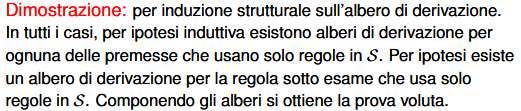
\includegraphics[width=0.75\linewidth]{dimderv.png}
    \caption{Dimostrazione del teorema sulla derivabilitá}
    \label{dimder}
\end{figure}

\paragraph{Or}
\begin{itemize}
    \item Introduzione \begin{mathpar}
        \inferrule*[Right = $\lor i_1$] {F_1} {F_1 \lor F_2}
    \end{mathpar}
    \begin{mathpar}
        \inferrule*[Right = $\lor i_2$] {F_2} {F_1 \lor F_2}
    \end{mathpar}
    Queste regole sono \textbf{altamente non invertibili}, quindi devono essere usata il piú tardi possibile nella dimostrazione.
    \item Eliminazione \begin{mathpar}
        \inferrule*[Right=$\lor e$] {F_1 \lor F_2 \\ F_3\inferrule*[vdots = 1.5 em] {}{[F_1]} \\ F_3\inferrule*[vdots = 1.5 em] {}{[F_2]} } {F_3}
    \end{mathpar}
    Quasta regola é parzialmente invertibile
\end{itemize}

\paragraph{Bottom ($\perp$)}
\begin{itemize}
    \item Introduzione: non esiste
    \item Eliminazione \begin{mathpar}
        \inferrule*[Right=$\perp_e$]{\perp}{F}
    \end{mathpar}
    questa regola é molto utilizzata nelle dimostrazioni per contaddizione perché porta a dei cicli giusti (essendo una regola invertibile) che non concludono (infatti posso sempre tornare a bottom con qualsiasi proposizione) ma che sono utili finché aggiungono ipotesi.
\end{itemize}

\paragraph{Top ($\top$)}
\begin{itemize}
    \item Introduzione: \begin{mathpar}
        \inferrule*[Right=$\top_i$]{ }{\top}
    \end{mathpar}
    (regola assioma)
    \item Eliminazione: inutile \begin{mathpar}
        \inferrule*[Right=$\top_e$]{\top \\ F}{F}
    \end{mathpar}
\end{itemize}

\paragraph{Implicazione ($\Rightarrow$)}
\begin{itemize}
    \item Introduzione: \begin{mathpar}
        \inferrule*[Right=$\Rightarrow_i$]{F_2 \inferrule*[vdots = 1.5 em]{}{[F_1]}}{F_1 \Rightarrow F_2}
    \end{mathpar}
    \item Eliminazione: \begin{mathpar}
        \inferrule*[Right = $\Rightarrow_e$]{F_1 \Rightarrow F_2 \\ F_1}{F_2}
    \end{mathpar}
    questa regole non é invertibile infatti non si ha nessuna garanzi che $F_1$ sia dimostrabile.
\end{itemize}
\paragraph{Not ($\neg$)} puó essere vista come $\neg F \equiv (F \Rightarrow\perp)$ quindi come caso particolare del bottom.
\begin{itemize}
    \item Introduzione: \begin{mathpar}
        \inferrule*[Right=$\neg_i$]{\perp \inferrule*[vdots = 1.5 em]{}{[F_1]}} {\neg F_1}
    \end{mathpar}
    \item Eliminazione: \begin{mathpar}
        \inferrule*[Right=$\neg_e$]{\neg F \\ F}{\perp}
    \end{mathpar}
    questa é un regola invertibile.
\end{itemize}

\paragraph{RAA (Riduzione ad assurdo)}
\begin{mathpar}
    \inferrule*[Right= $RAA$]{\perp \inferrule*[vdots = 1.5 em]{}{[\neg F]}} {F}
\end{mathpar}

\paragraph{EM (principio del terzo escluso)}
\begin{mathpar}
    \inferrule*[Right = $\lor_e$] {A \lor \neg A \\ F \inferrule*[vdots = 1.5 em]{}{[A]} \\ F \inferrule*[vdots = 1.5 em]{}{[\neg A]}} {F}
\end{mathpar}

\section{Semantica classica della logica proposizionale}
In qesta sezione si studierá il concetto di valere (dato dalla semantica classica) ovvero l'associazione di un valore di veritá ad ogni denotazione di ogni connotazione. Alcuni termini importanti:
\begin{figure}[H]
    \centering
    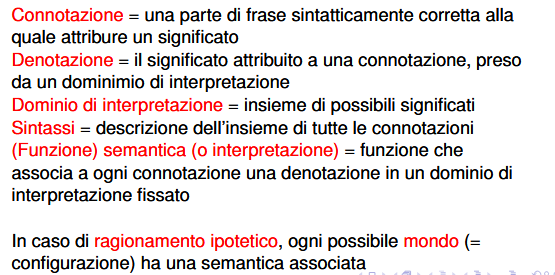
\includegraphics[width=0.75\linewidth]{def.png}
    \caption{Definizioni di termini importanti}
    \label{def}
\end{figure}

In altre parole iol \textbf{mondo} determina il valore di veritá delle variabili proposizionali, per cui ci saranno tanti mondi quante le possibili combinazioni dei possibili valori di veritá delle varie variabili proposizionali.

\subsection{Visione filosofica della veritá}
\begin{enumerate}
    \item Ogni enunciato é vero o falso.
    \item Un enunciato non puó essere vero e falsdo nello stesso momento.
    \item Il valore di veritá non muta.
    \item Il valore di veritá di un enunciato é sempre determinato.
\end{enumerate}

Dai primi due punti si ottiene il \textbf{Dominio di interpretazione classico} ovvero che i valori di veritá appartengono all'insieme $\{0,1\}$, gli ultimi due invece implicano l'esistenza di una \textbf{Funziona di interpretazione (o mondo)} ovvero una funzione che $\{A,B,C,...\} \rightarrow \{0,1\}$. Le interpretazioni sono indicate con $v,v',v_1,v_2...$

\subsection{Definizione della sematica delle formule}
Una formula sintatticamente corretta non é una stringa ma un \textbf{albero di sintassi astratta} la cui veritá si puó calcolare attraverso la \textbf{ricorsione strutturale} questo perché ogni nodo di un albero puó essere considerato un ulteriore sotto-albero.
\paragraph{Definizione} data un'interpretazione (modno) $v$, la semantica $[[.]]^v:F \rightarrow \{0,1\}$ é definita per ricorsione come segue":
\begin{itemize}
    \item $[[\perp]]^v = 0$
    \item $[[\top]] = 1$
    \item $[[A]]=v(A)$
    \item $[[\neg F]]^v= 1 - [[F]]^v$
    \item $[[F_1 \land F_2]]^v = min([[F_1]]^v,[[F_2]]^v)$
    \item $[[F_1 \lor F_2]]^v = max([[F_1]]^v,[[F_2]]^v)$
    \item $[[F_1 \Rightarrow F_2]] = max(1-[[F_1]]^v,[[F_2]]^v)$
\end{itemize}

\section{Conseguenza logica}
In questa sezione si approfondirà la nozione di conseguenza logica, centrale nelle dimostrazione; essa é definita come $\Gamma \vDash F \Leftrightarrow \forall v, [[G]]^v = 1, \forall G \in \Gamma \Rightarrow [[F]]^v =1$.

Questa definizione ci dice diverse cose:
\begin{itemize}
    \item $min \{[[G]]^v | G\in \Gamma\} \le [[F]]^v$
    \item se $\Gamma \vDash F$ e $\Gamma = F_1, F_2,...$ allora $[[F]]^v = 1$ in quella che è l'intersezione di tutti i mondi rappresentati da $F_1, F_2,...$ tutti sottoinsiemi di tutti i mondi possibili
\end{itemize}

\section{Fallimento della completezza della logica classica}
Ogni teoria logica si può dire 
\begin{itemize}
    \item \textbf{Corretta} se $\forall\Gamma, F.\Gamma \vdash F \Rightarrow \Gamma\vDash F$ (ovvero da senso alle dimostrazioni).
    \item \textbf{Completa} se $\forall\Gamma,F.\Gamma\vDash F \Rightarrow\Gamma\vdash F$ (molto rari i casi in cui una toria lo sia).
\end{itemize}
La deduzione naturale è \textbf{corretta} ma \textbf{non completa}: le due tautologie $\neg (\neg A) = A$ e $\vDash A \lor \neg A$ non si possono dimostrare con questa logica. Per cui ci sono due modi di ovviare a questi problemi:
\begin{enumerate}
    \item Aggiungere la \textbf{RAA} per rendere la logica classica completa
    \item Cambiare la logica in cui si sta lavorando in modo tale che le regole siano complete rispetto ad essa.
\end{enumerate}
\paragraph{Dimostrazioni di completezza e invertibilitá delle formule di inferenza}
Si tratta di verificare, tramite le definizioni della semantica delle formule se una volta poste come vere le premesse la conclusione é vera. Pe ersempio ecco la dimostrazione di correttezza e invertibilitá della regola di introduzione dell'and:
\begin{itemize}
    \item \textbf{Correttezza}: $F_1,F_2 \vDash F_1 \land F_2 = \forall v.(\forall G\in\{F_1,F_2\}.[[G]]^v=1)\Rightarrow[[F_1 \land F_2]]^v=1$ dunque, se $[[F_1]]^v=[[F_2]]^v=1$, allora $[[F_1\land F_2]]^v=min\{[[F_1]]^v,[[F_2]]^v\}=1$
    \item \textbf{Invertibilitá }: $F_1 \land F_2 \vDash F_i, i\in\{1,2\}$ semplicemente $[[F_1\land F_2]]^2 = min\{[[F_1]]^v,[[F_2]]^v\} = 1$, quindi $[[F_1]]^v=[[F_2]]^v=1$
\end{itemize}


\section{Semantca intuizionista}
É la semantica dell'evidente ovvero di ció che é conoscibile in modo diretto e calcolabile, dunque per sapere che qualcosa esiste non é piú possible dimostrarne solo l'esistenza ma bisogna trovare un algoitmo per trovare quella determinata "cosa", per esempio per dimostrare infiniti numeri primi bidsogna trovare un algormitmo che permetta, dato qualsiasi numero, di stabilire se sia primo o meno. Una semantica equivalente a questa é quella di Brouwer-Heyting-Kolmogorov:
\begin{itemize}
    \item Una \textbf{Formula} é una descrizione di un problema.
    \item La \textbf{Denotazione} di una formula é l'insieme di algoritmi conosciutio per risolvere il problema della formula.
    \item L'insieme vuoto é un problema senza soluzioni, mentre un insieme non vuoto é un problema con almeno una soluzione.
    \item Un \textbf{Connettivo} descrive un problema a partire da altri problemi
    \item La \textbf{Denotazione di un Connettivo} é l'insieme di algoritmi che risolvono il problema complesso a partire da algoritmi che risolvono i problemi semplici.
\end{itemize}

\paragraph{Semantca}
\begin{itemize}
    \item $[[A]]^v = v(A)$
    \item $[[\perp]]^v = \emptyset$
    \item $[[\top]]^v=\{*\}$ (problema banale e * lo risolve)
    \item $[[F \land G]]^v = [[F]]^v \times[[G]]^v$ (prodotto cartesiano)
    \item $[[F \lor G]]^v = [[F]]^v \bigoplus[[G]]^v$ (unione disgiunta $<b,\pi>$ tali che se$ b = 0$ allora $\pi$ risolve F se invece $b=1$ allora $\pi$ risolve G
    \item $[[F \Rightarrow G]]^v = [[G]]^{v[[F]]^v}$
    \item Non esiste il terzo escluso
    \item $\not\vDash \neg\neg A \Rightarrow A$
    \item \textbf{Teorema} $\forall\Gamma, F. \Gamma \vDash F$ in logica intuizionista $\Rightarrow \Gamma\vDash F$ anche in logica classica
\end{itemize}

\paragraph{Teoremna correttezza} $\forall\Gamma.F. \Gamma \vdash F$ senza ricorrere alla \textbf{RAA} allora $\Gamma \vDash F$ in \textit{logica proposizionale intuizionista}.
\paragraph{Teorema completezza (debole)} $\forall\Gamma. F. \Gamma\vDash F$ in logica intuizionista allora $\Gamma \vdash F$ senza la \textbf{RAA}.

\section{Logica del prim'ordine}
Serve perché in aluni casi la logica classica non basta, per esempio servirá a poter usare i connettivi $\forall,\exists$ in deduzione naturale e poter fare cosí le stesse dimostrazioni della teoria degli insiemi.
\begin{itemize}
    \item \textbf{Formule} connotazioni che \textbf{denotano valori di veritá} \begin{itemize}
        \item \textbf{predicati}: $P^n$
        \item \textbf{connettivi}: $\land, \lor,\Rightarrow,\perp,\top$
        \item \textbf{quantificatori}: $\forall,\exists$
    \end{itemize}
    \item \textbf{Termini} denotano \textbf{elementi del domini di interpretzione} \begin{itemize}
        \item \textbf{variabili}: $x,t$
        \item \textbf{costanti}: c
        \item \textbf{funzioni}: $f^n(t_1,...,t_n)$ [n = arietá: numero di parametri necessari]
    \end{itemize}
\end{itemize}

Rispetto alla logica proposizionale smbrano essersi perse le variabili proposizionali ma esse possono essere implementate tramite \textbf{proprietá di arietá 0} ovvero un valore di verita che non dipende (e non prende) input [\textit{variabili proposizionali generalizzate}], la \textbf{teoria degli insiemi}, invece, é contenuta nella logica del priom'ordine
\subsection{Semantica}
\begin{itemize}
    \item Ogni simbolo di costante deve essee associato ad elemento di A [\textit{dominio di nterpretabilitá}], per esempio $[[c]]^v\in A \to [[\pi]]^v=2$ con v che sceglie $\mathbb{N}$ come A.
    \item Una funzione prende \textit{n. elementi} di A e ritorna un elmento di A.
    \item Un \textbf{predicato} prende \textit{n. elementi} e ritorna un valore di veritá.
    \item $[[\forall x.F]]^v=1 \Leftrightarrow v(F)=1, \forall x \in A$
    \item $[[\exists x.F]]^v=1 \Leftrightarrow \exists X \in A | v(A) \Rightarrow v(F) = 1$
\end{itemize}

\subsection{Quantificatori}
I quantificatori, in generale, sono casi particolari di \textbf{binder} ovvero legano le singole variabili agli scope. per come funzionano hanno un problema comune in qualisasi tipo di implementazione ovvero lo \textbf{shadowing}, per esempio analizziamo la formula $\forall x.P(x) \land \exists x. Q(x)$ la x dei due quantificatori é simbolicamente la stessa ma non é detta che sia sempre la stessa. Dunque i quantificatori creano uno \textit{scope} della variabile a cui sono legati e se la variabile viene legata ad un altro quantificatore si apre un nuovo scope che oscura il valore precedente della variabile. Per capire quali variabili sono legati a quali scope oppure quali sono \textbf{variabili libere} si puó fare il \textbf{diagramma di legame} di una formula logica che consiste nel indicare con una freccia a quale quantificatore ogni variabile é legata, nel caso in cui non lo sia essa é una \textit{variabile libera}. Un altro modo di calcolare quali siano le variabili libere si puó ricorrere anche alla \textit{ricorsione strutturale}:
\begin{itemize}
    \item $F.V.(x) := \{x\}$
    \item $F.V.(f^n(t_1,...,t_n))=F.V.(t_1) \cup...\cup F.V.(t_n)$
    \item $F.V.(\perp)=F.V.(\top) =\emptyset$ 
    \item $F.V.(\neg F) = F.V.(F)$
    \item $F.V.(A\land B) = F.V.(A\lor B) =F.V.(A\Rightarrow B)=F.V.(A)\cup F.V.(B)\land F.V.(\forall x.P)=F.V.(\exists x.P)=F.V.(P)/\{x\}$ (cattura x)
\end{itemize}
Avere lo stesso diagramma di legame é sinonimo di equivalente con tutte le corrispettive proprietá, due formule \textbf{equivalenti} di dicono $\alpha$-convertibili ($\equiv_\alpha$).
\paragraph{Sostituzione}
In questa approfondiremo le \textbf{funzioni di sostituzione} ovvero funzioni che permettono di sostituire con un termine $t$ ad una variabile precedentemente legata, nelle dimostrazioni da questo punto in poi molti errori occorreranno per errate sostituzioni. Di seguito le formule per una giusta \textbf{sostituzione}:
\begin{itemize}
    \item $x[t/x]=t$
    \item $y[t/x]=y$
    \item $f^n(t_1,...,t_n)[t/x]=f^n(t_1[t/x],...,t_n[t/x])$
    \item $P^n(t_1,...,t_n)[t/x]=P^n(t_1[t/x],...,t_n[t/x])$
    \item $\perp[t/x]=\perp$
    \item $\top[t/x]=\top$
    \item $(\neg F)[t/x]=\neg(F[t/x])$
    \item $(A\land B)[t/x]=A[t/x]\land B[t/x]$
    \item $(A\lor B)[t/x]=A[t/x]\lor B[t/x]$
    \item $(A\Rightarrow B)[t/x]=A[t/x]\Rightarrow B[t/x]$
    \item $\forall x.P[t/x]=\forall x.P$
    \item $\exists  x.P[t/x]=\exists x.P$
\end{itemize}
\subsection{Deduzione naturale per la logica del prim'ordine}
\paragraph{Per ogni}
\begin{itemize}
    \item Introduzione \begin{mathpar}
        \inferrule*[Right = $\forall_i$ con $y \in F.V.(foglie)$]{P[y/x]}{\forall x.P}
    \end{mathpar}
    Questa regola é corretta e invertibile.
    \item Eliminazione \begin{mathpar}
        \inferrule*[Right = $\forall e$]{\forall x.P}{P[y/x]}
    \end{mathpar}
    Questa regola non é invertibile
\end{itemize}
\paragraph{Esiste}
\begin{itemize}
    \item Introduzione \begin{mathpar}
        \inferrule*[Right = $\exists_i$]{P[y/x]}{\exists x.P}
    \end{mathpar}
    Questa regola é fortemente non invertibile.
    \item Eliminazione \begin{mathpar}
        \inferrule*[Right = $\exists e$ con $y \in F.V.(C) \cup F.V.(foglie)$]{\exists x.P \\ C \\ \inferrule*[vdots = 1.5 em]{}{P[y/x]}}{C}
    \end{mathpar}
    Questa regolaw é invertibile
\end{itemize}


\end{document}